\subsubsection{Front-end}

\par Vue.js implementa il pattern architetturale MVVM (Model-View-ViewModel), una declinazione del pattern Model-View-Controller (MVC). L’MVVM viene integrato nativamente attraverso il modo in cui Vue gestisce i dati, la logica e l'interfaccia utente. Il ViewModel è un oggetto che sincronizza il Model e la View. Ogni istanza di Vue è un ViewModel.

\begin{figure}[H]
  \centering
  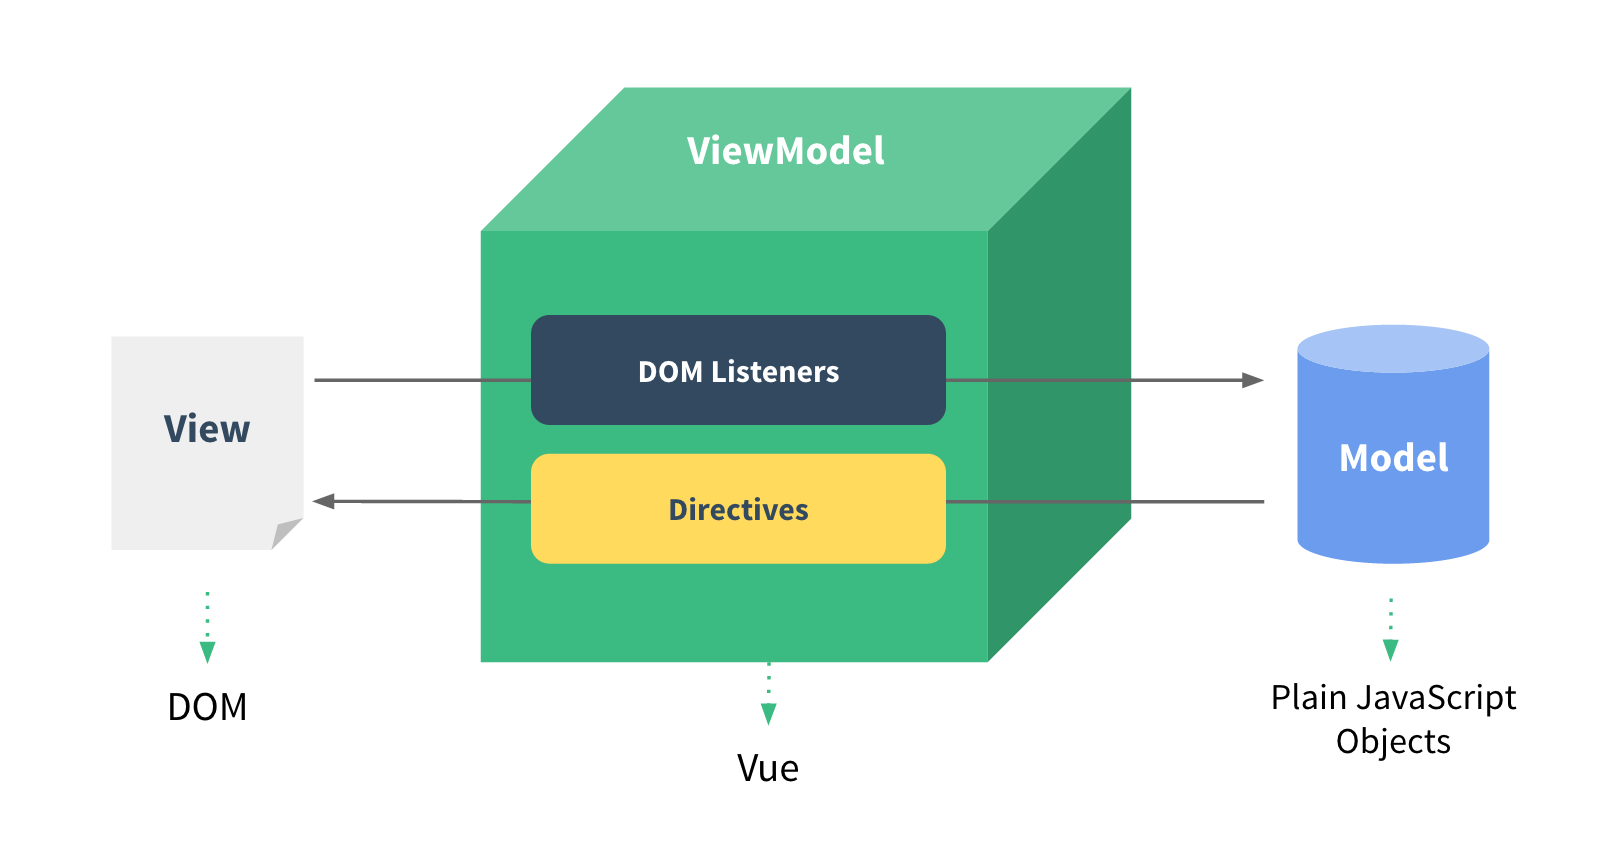
\includegraphics[width=0.95\textwidth]{assets/Frontend/architettura_mvvm.png}
  \caption{Model-View-ViewModel (MVVM)}
\end{figure}

\par Il pattern MVVM comprende tre layer, ciascuno con un ruolo specifico:
\begin{itemize}
  \item \textbf{Model}: è responsabile della gestione dei dati e della logica di business. In Vue.js, il Model è tipicamente rappresentato da semplici oggetti JavaScript (plain JavaScript objects) o data model objects (oggetti più strutturati) che diventano reattivi quando utilizzati dalle istanze di Vue. Inoltre, Vue offre soluzioni per la gestione centralizzata dello stato, come Vuex e Pinia;
  \item \textbf{View} (Presentation layer): è responsabile della presentazione dei dati all'utente. Descrive la struttura del DOM (Document Object Model). La View è rappresentata dal template, che utilizza una sintassi HTML arricchita con binding e direttive specifiche per riflettere i cambiamento di stato. L'interfaccia viene aggiornata dinamicamente quando cambiano i dati del modello;
  \item \textbf{ViewModel}: è il layer che collega il Model e la View. Ha il compito di gestire le interazioni dell'utente e sincronizzare i dati con la View. Il ViewModel è rappresentato dalle istanze di Vue. Oltre a sincronizzare il Model e la View, il ViewModel garantisce una chiara separazione tra i dati e la logica di presentazione.
\end{itemize} 

\begin{figure}[H]
  \centering
  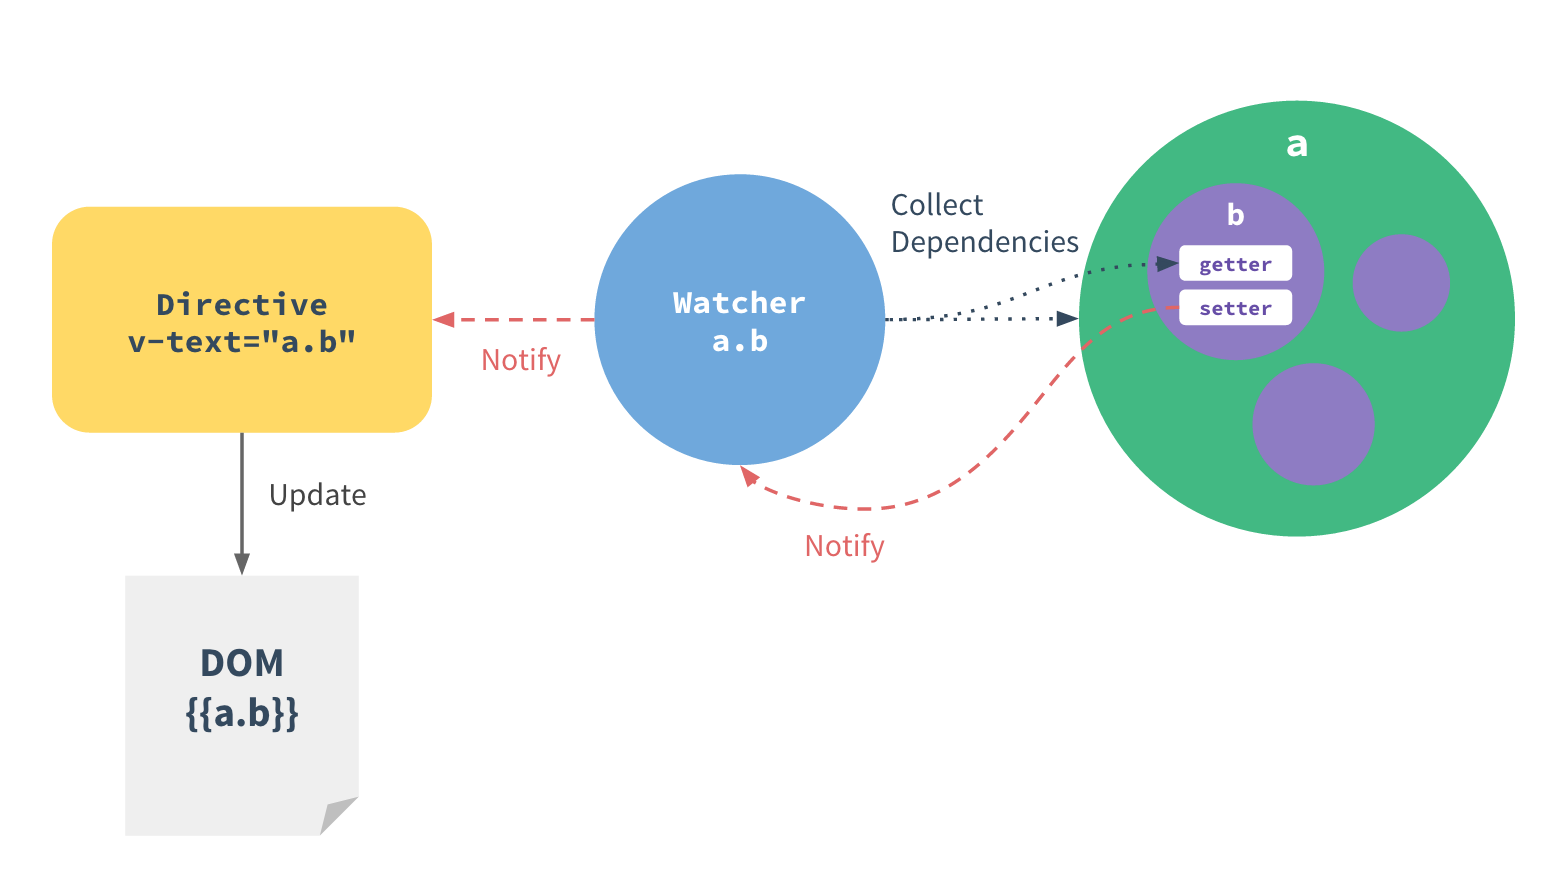
\includegraphics[width=0.95\textwidth]{assets/Frontend/overview_mvvm.png}
  \caption{Funzionamento del pattern MVVM}
\end{figure}

\par Vue.js implementa due concetti fondamentali:
\begin{itemize}
  \item \textbf{Reattività}: la reattività è un meccanismo che permette di aggiornare dinamicamente la View quando cambiano i dati del Model. I dati reattivi sono oggetti che vengono osservati da Vue. La differenza rispetto ai normali oggetti JavaScript è che Vue è in grado di intercettare l'accesso e la modifica di tutte le proprietà di un oggetto reattivo;
  \item \textbf{Composition API}: permette di suddividere la logica di un componente in funzioni riutilizzabili. La Composition API migliora la riusabilità, l'organizzazione e la manutenibilità del codice. Inoltre, la Composition API risolve alcune limitazioni della Options API, che emergono quando la logica di un singolo componente supera una determinata soglia di complessità.
\end{itemize}

\vspace{0.5\baselineskip}
\par La struttura organizzativa del front-end segue le convenzioni definite dal framework Vue.js, con alcune modifiche e personalizzazioni per migliorare la riusabilità, la manutenibilità e l'usabilità. Il front-end è suddiviso nelle seguenti cartelle:

\begin{minipage}{\textwidth}
  \dirtree{%
    .1 frontend.
    .2 public.
    .3 themes.
    .3 icons.
    .2 src.
    .3 assets.
    .3 components.
    .4 layout.
    .3 composables.
    .3 locales.
    .3 router.
    .3 services.
    .3 types.
    .3 views.
  }
\end{minipage}

\vspace{0.5\baselineskip}
\par Di seguito è riportata una breve descrizione delle cartelle principali:
\begin{itemize}
  \item \textbf{public}: contiene le icone e i temi utilizzati nell'applicazione;
  \item \textbf{src}: contiene il codice sorgente e gli assets.
\end{itemize}

\vspace{0.5\baselineskip}
\par La cartella \textit{src} è suddivisa nelle seguenti sottocartelle:
\begin{itemize}
  \item \textbf{assets}: contiene i file statici, come immagini, font e fogli di stile;
  \item \textbf{components}: contiene i componenti Vue riutilizzabili da più viste;
  \item \textbf{composables}: contiene le funzioni riutilizzabili;
  \item \textbf{locales}: contiene i file \glossario{JSON} di traduzione;
  \item \textbf{router}: contiene le definizioni delle route dell'applicazione. La definizione di una route comprende l'URL o il percorso che l'utente deve inserire nel browser per accedere alla route. Inoltre, specifica quale componente deve essere caricato quando l'utente accede a quel percorso;
  \item \textbf{services}: contiene funzioni di utilità e servizi per la comunicazione con il back-end;
  \item \textbf{types}: contiene le definizioni dei tipi e delle interfacce per un'API basata su OpenAPI;
  \item \textbf{views}: contiene le viste dell'applicazione. Una vista è un componente principale che può essere suddiviso in sottocomponenti, disponibili nella cartella \textit{components}. In genere, le view rappresentano pagine o sezioni centrali e sono gestite dal router di Vue.
\end{itemize}
